\documentclass[12pt,letterpaper]{exam}
\usepackage[lmargin=1in,rmargin=1in,tmargin=1in,bmargin=1in]{geometry}
\usepackage{../style/exams}

% -------------------
% Course & Exam Information
% -------------------
\newcommand{\course}{MAT 108: Exam 1}
\newcommand{\term}{Fall -- 2021}
\newcommand{\examdate}{10/12/2021}
\newcommand{\timelimit}{85 Minutes}

\setbool{hideans}{true} % Student: True; Instructor: False

% -------------------
% Content
% -------------------
\begin{document}

\examtitle
\instructions{Write your name on the appropriate line on the exam cover sheet. This exam contains \numpages\ pages (including this cover page) and \numquestions\ questions. Check that you have every page of the exam. Answer the questions in the spaces provided on the question sheets. Be sure to answer every part of each question and show all your work. If you run out of room for an answer, continue on the back of the page --- being sure to indicate the problem number.} 
\scores
\bottomline
\newpage

% ---------
% Questions
% ---------
\begin{questions}

% Question 1
\newpage
\question[12] Consider the following relations below:

	\[
	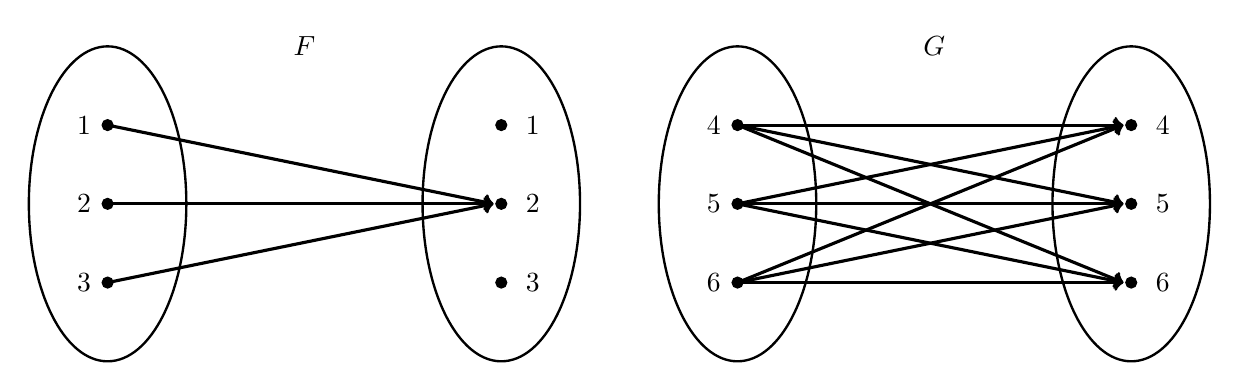
\begin{tikzpicture}
	\node at (2.5,2) {$F$};
	% Ellipses
	\draw[line width=0.03cm] (0,0) circle (1 and 2);
	\draw[line width=0.03cm] (5,0) circle (1 and 2);
	
	% Nodes
	\draw[fill=black] (0,1) circle (0.07);
	\draw[fill=black] (0,0) circle (0.07);
	\draw[fill=black] (0,-1) circle (0.07);
	
	\draw[fill=black] (5,1) circle (0.07);
	\draw[fill=black] (5,0) circle (0.07);
	\draw[fill=black] (5,-1) circle (0.07);
	
	% Arrow
	\draw[line width=0.04cm,->] (0,1) -- (4.9,0);
	\draw[line width=0.04cm,->] (0,0) -- (4.9,0);
	\draw[line width=0.04cm,->] (0,-1) -- (4.9,0);
	
	% Labels
	\node at (-0.3,1) {$1$};
	\node at (-0.3,0) {$2$};
	\node at (-0.3,-1) {$3$};
	
	\node at (5.4,1) {$1$};
	\node at (5.4,0) {$2$};
	\node at (5.4,-1) {$3$};
	
	\tikzset{shift={(8,0)}}
	%
	\node at (2.5,2) {$G$};
	% Ellipses
	\draw[line width=0.03cm] (0,0) circle (1 and 2);
	\draw[line width=0.03cm] (5,0) circle (1 and 2);
	
	% Nodes
	\draw[fill=black] (0,1) circle (0.07);
	\draw[fill=black] (0,0) circle (0.07);
	\draw[fill=black] (0,-1) circle (0.07);
	
	\draw[fill=black] (5,1) circle (0.07);
	\draw[fill=black] (5,0) circle (0.07);
	\draw[fill=black] (5,-1) circle (0.07);
	
	% Arrow
	\draw[line width=0.04cm,->] (0,1) -- (4.9,1);
	\draw[line width=0.04cm,->] (0,1) -- (4.9,0);
	\draw[line width=0.04cm,->] (0,1) -- (4.9,-1);
	\draw[line width=0.04cm,->] (0,0) -- (4.9,1);
	\draw[line width=0.04cm,->] (0,0) -- (4.9,0);
	\draw[line width=0.04cm,->] (0,0) -- (4.9,-1);
	\draw[line width=0.04cm,->] (0,-1) -- (4.9,1);
	\draw[line width=0.04cm,->] (0,-1) -- (4.9,0);
	\draw[line width=0.04cm,->] (0,-1) -- (4.9,-1);
	
	% Labels
	\node at (-0.3,1) {$4$};
	\node at (-0.3,0) {$5$};
	\node at (-0.3,-1) {$6$};
	
	\node at (5.4,1) {$4$};
	\node at (5.4,0) {$5$};
	\node at (5.4,-1) {$6$};
	\end{tikzpicture}
	\] \pspace

	\begin{minipage}[b]{0.49\textwidth}
	\centering
	\begin{tabular}{c|rcc|r}
	$x$ & $H(x)$ & \hspace{1cm} & $x$ & $J(x)$ \\ \cline{1-2} \cline{4-5}
	$1$ & $-1$ & & $5$ & $0$ \\
	$2$ & $2$ & & $6$ & $0$ \\
	$3$ & $3$ & & $8$ & $1$ \\
	$4$ & $-4$ & & $9$ & $0$ \\
	$5$ & $6$ & & $5$ & $1$
	\end{tabular}
	\end{minipage}
	\begin{minipage}[b]{0.49\textwidth}
	\[
	\begin{aligned}
	K(x)&:= 18.87x - 24 \\[0.6cm]
	L(x)&:= 2x(1 - x^8)
	\end{aligned}
	\]
	\end{minipage} \pvspace{0.6cm}
	
Determine if each of the relations given above is a function. If the relation is a function, write `T' (True) and if the relation is \emph{not} a function, write `F' (False): \pspace

	\begin{enumerate}[(a)]
	\item \uans{1.6cm}: $F(x)$ \pvspace{0.3cm}
	\item \uans{1.6cm}: $G(x)$ \pvspace{0.3cm}
	\item \uans{1.6cm}: $H(x)$ \pvspace{0.3cm}
	\item \uans{1.6cm}: $J(x)$ \pvspace{0.3cm}
	\item \uans{1.6cm}: $K(x)$ \pvspace{0.3cm}
	\item \uans{1.6cm}: $L(x)$
	\end{enumerate}





% Question 2
\newpage
\question[10] As accurately as possible, plot the solution set to the system of inequalities
	\[
	\begin{aligned}
	\frac{1}{3}\,x + 1&\geq y  \\
	12x + 2y &\leq 3 
	\end{aligned}
	\]
	\vfill
	\[
	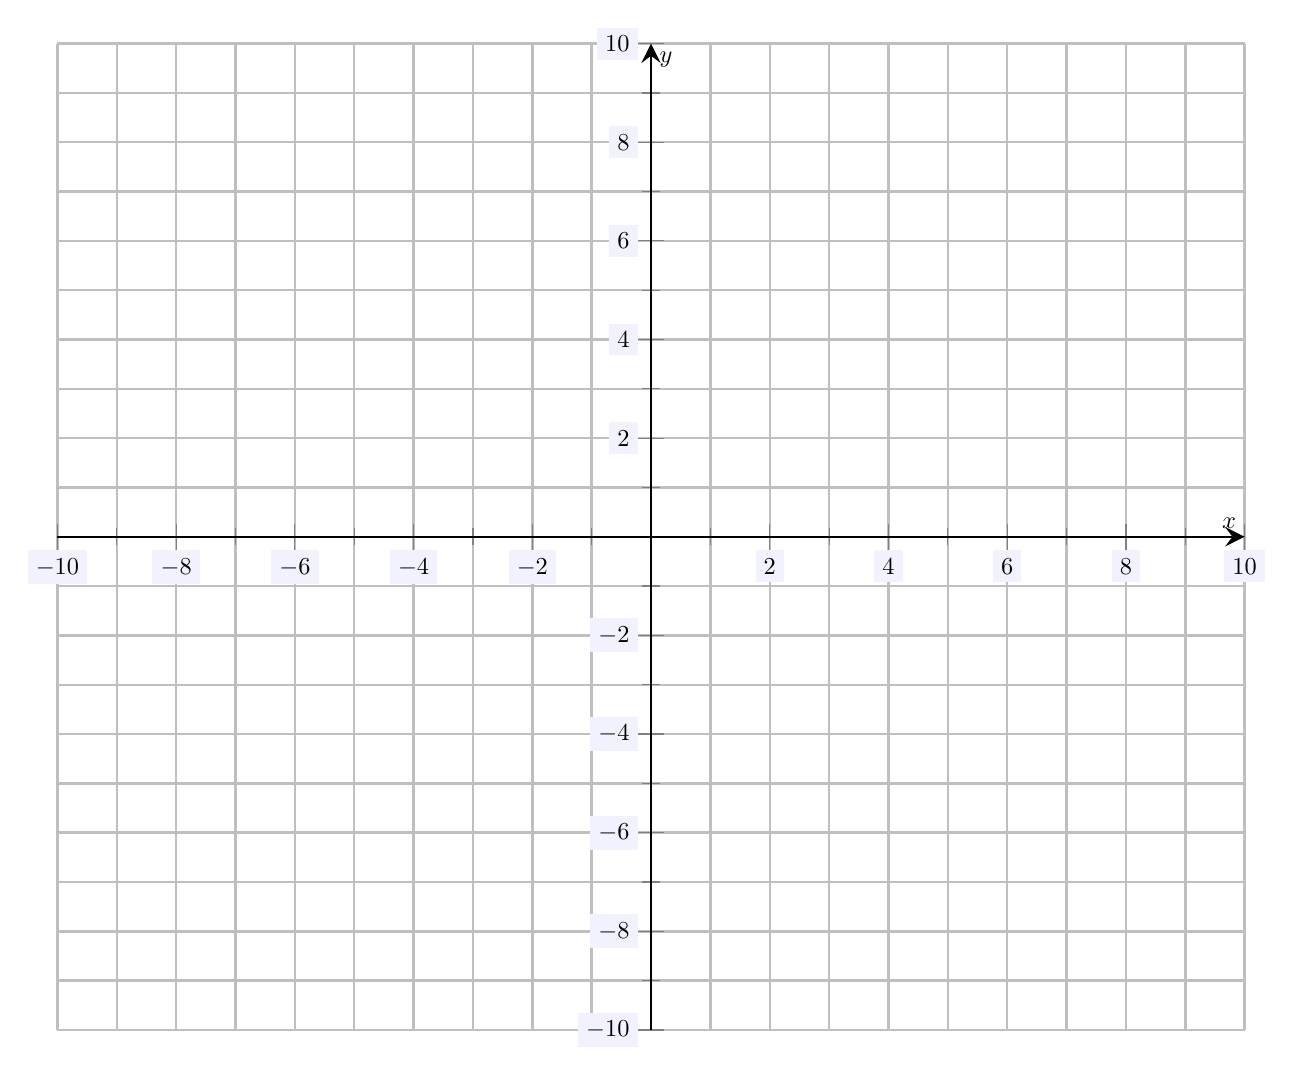
\begin{tikzpicture}[scale=2.2,every node/.style={scale=0.4}]
	\begin{axis}[
	grid=both,
	axis lines=middle,
	ticklabel style={fill=blue!5!white},
	xmin= -10, xmax=10,
	ymin= -10, ymax=10,
	xtick={-10,-8,...,10},
	ytick={-10,-8,...,10},
	minor tick = {-10,-9,...,10},
	xlabel=\(x\),ylabel=\(y\),
	]

	\end{axis}
	\end{tikzpicture}
	\]





% Question 3
\newpage
\question Consider the function given by $\ell(x)= 15x - 60$. \pspace

\begin{parts}
\part[2] Is this function linear? Explain. \pvspace{3cm}
\part[2] Describe the graph of the function. \pvspace{3cm}
\part[3] What is the $x$-intercept for this function? \vfill
\part[3] What is the $y$-intercept for this function? \vfill
\end{parts}





% Question 4
\newpage
\question A company produces widgets. The cost function associated to production is $C(x)= 5x + 120$ and the revenue function for this product is $R(x)= 10x$. \pspace

\begin{parts}
\part[2] What are the fixed costs for production? \pvspace{4cm}
\part[2] How much does each widget cost to produce? \pvspace{4cm}
\part[2] How much does the company sell each widget for? \pvspace{4cm}
\part[6] What is the breakeven point?
\end{parts}





% Question 5
\newpage
\question[10] The following matrix represents an augmented system in reduced row echelon form. 
	\[
	\begin{pmatrix}
	1 & 0 & 5 & 0 & 0 & 0 & 1 \\
	0 & 1 & 0 & 0 & 0 & 0 & -2 \\
	0 & 0 & 0 & 1 & -7 & 0 & -2 \\
	0 & 0 & 0 & 0 & 0 & 1 & 3 \\
	\end{pmatrix}
	\] 
Find the set of solutions to the corresponding system of equations. 





% Question 6
\newpage
\question Define the following matrix:
	\[
	A= \left(
	\begin{array}{rrrr}
	2 & 0 & -5 & 1 \\
	1 & 2 & 1 & 0 \\
	-1 & 0 & -1 & 2 \\
	0 & 0 & 4 & -3 \\
	\end{array} \right)
	\]

\begin{parts}
\part[6] Compute $\det A$. \vfill
\part[6] Does $A^{-1}$ exist? Explain. \pvspace{5cm}
\end{parts}





% Question 7
\newpage
\question Consider the matrix equation $A\mathbf{x}= \mathbf{b}$ given by
	\[
	\begin{pmatrix}
	-6 & 8 \\
	-5 & 7
	\end{pmatrix}
	\begin{pmatrix}
	x_1 \\
	x_2 
	\end{pmatrix}=
	\begin{pmatrix}
	-2 \\
	1
	\end{pmatrix}
	\] \pspace

\begin{parts}
\part[6] Find the inverse of the matrix $A$ in the system above. \vfill

\part[6] Use $A^{-1}$ to solve the matrix equation. \vspace{7cm}
\end{parts}





% Question 8
\newpage
\question[12] Compute the following:
	\[
	\begin{pmatrix}
	1 & 0 & -1 & 1 \\
	1 & 4 & 1 & 5 \\
	0 & -2 & -2 & 1 
	\end{pmatrix}
	\begin{pmatrix}
	1 & 1 \\
	2 & 2 \\
	0 & -1 \\
	1 & 0
	\end{pmatrix}
	\]





% Question 9
\newpage
\question[10] Consider the system of equations represented by the augmented matrix
	\[
	\begin{pmatrix}
	2 & 4 & 6 \\
	-1 & -5 & 3
	\end{pmatrix}
	\]
By placing the matrix in reduced row echelon form, solve the corresponding system of equations. 


\end{questions}
\end{document}